\chapter{Capstone: A Wrist-Worn Gesture Controller for Instruments}

Every chapter of this book has carried the same quiet promise: that the
geometry of frequency --- signals as vectors, the Fourier transform as a set of
projections, convolution as a sliding overlap, filtering as turning knobs in the
spectrum --- was not abstract decoration but a toolkit for building something
real. This is the chapter where we cash that promise. We are going to build a
\emph{wrist/forearm-worn finger-gesture controller}: a band you wear on your arm
that detects which finger you just moved, reads how your wrist is oriented and
moving, and turns all of that into MIDI --- the language synthesizers and
digital audio workstations speak. Play it like an instrument: lift the index
finger to trigger a note, twist your wrist to bend the pitch, curl the ring
finger for a chord, spread your fingers to open a filter.

Finger movement \emph{is} detectable from the wrist, and this chapter shows how
without a shred of machine learning. The trick is not a clever model; it is
\emph{calibration}. Each finger movement, sensed through the forearm tendons or
muscle electrical activity, leaves a repeatable signature on a band of sensors.
A short guided enrollment --- the user wiggles each finger a few times --- records
those signatures as per-user \emph{templates}. Live play is then a direct match:
compare the current sensor reading to the templates and fire the nearest one.
Calibration is the heart of the instrument; everything else is conditioning the
signals so the match is clean.

We open by separating what the wrist genuinely reveals from the one thing it
genuinely hides, then walk the entire pipeline end to end --- sensor choice,
wiring, the thin-node-plus-phone architecture, sampling, de-noising, the
per-finger calibration routine, windowing, feature extraction, template
matching, latency budgeting, and MIDI mapping --- using the very techniques the
earlier chapters built. We close with a real bill of materials, a frank
accuracy-and-difficulty box, the failure modes that will actually bite you, and
an upgrade path toward true continuous finger tracking.

\section{What the wrist reveals, and the one thing it hides}
\label{ch41:goal}

Let us draw the line precisely, because the difference between a project that
works and one that disappoints is almost always set in the first five minutes
by an over-promise --- or, just as bad, by an under-promise that throws away
something real.

Here is the achievable part, stated plainly: \textbf{which finger moved is
recoverable from a wrist or forearm band}, with per-user calibration. Your
finger flexors and extensors sit in the forearm, right under the band. When you
move a finger, the responsible muscle contracts and \emph{bulges}, pressing on
the skin (\emph{force myography}, FMG), and it emits an electrical burst
(\emph{surface electromyography}, sEMG). Different fingers recruit different
muscles, so each finger movement paints a different \emph{spatial pattern}
across a ring of sensors. Those patterns are repeatable enough, once calibrated
to your arm, that a direct match identifies the finger. WristFlex did exactly
this for finger pinches; the build here extends it with more sensing channels
and a richer calibration.

\begin{trapbox}
\textbf{The one genuinely hard thing: continuous per-joint finger \emph{angles}
cannot be recovered from the wrist.} Detecting \emph{that} the index finger
moved is easy; reconstructing the exact bend angle of each knuckle, continuously,
is not. A wrist IMU measures the acceleration and angular velocity \emph{of the
wrist}, and finger motion produces almost no inertial signature there. Even the
muscle sensors give a low-dimensional pressure/voltage pattern, not the dozen-odd
joint angles of the hand --- the mapping is underdetermined. So we read
\emph{discrete finger movements} (reliable) and \emph{wrist orientation}
(reliable), and we leave continuous joint angles to finger-worn sensors
(Section~\ref{ch41:upgrade}). Everything a player actually needs to perform ---
trigger notes by finger, shape them by wrist --- lives on the achievable side
of that line.
\end{trapbox}

So the instrument has two cooperating channels:

\begin{enumerate}
  \item \textbf{Per-finger movement detection} --- ``index,'' ``middle,''
        ``ring,'' ``fist,'' ``spread,'' ``rest'' --- from the FMG or sEMG band,
        matched against per-user templates built during enrollment. This answers
        \emph{which finger / which gesture}.
  \item \textbf{Continuous expressive control from the wrist} --- pitch bend from
        wrist tilt, modulation from roll, intensity from how hard and fast you
        moved --- from the IMU, where it genuinely shines. This answers
        \emph{how}.
\end{enumerate}

Combine the two and you have a real instrument: the muscle/tendon band says
\emph{which note and articulation}, the IMU says \emph{how high, how much
vibrato, how loud}. That division of labor is the whole design.

\begin{goalbox}
The wrist tracker we have been pointing at since Chapter~1 is a
\emph{finger-gesture-plus-expression} controller: a calibrated set of finger
movements (from FMG and sEMG) selecting and gating notes, continuously
modulated by wrist orientation and motion (from the IMU). There is \textbf{no
machine-learning model} anywhere in it. The method is direct --- a guided
enrollment records each finger's signature, and live detection matches the
current signal to those templates. Everything in this book --- sampling,
anti-alias filtering, windowing, the FFT, spectral and time-domain features,
sensor fusion, correlation and distance in feature space, latency budgeting ---
is exactly what turns the raw sensor streams into expressive, low-latency MIDI.
This chapter is the assembly.
\end{goalbox}

\begin{aestheticbox}
\textbf{More than a Fitbit, and not by adding a brain.} A Fitbit-class wearable
reads heart rate, steps, and sleep --- bulk-body signals. It cannot tell which
finger you moved, because it neither sits over the finger muscles nor samples
fast enough to catch a contact event. Our band does three things a fitness
tracker does not: it places a sensor array \emph{over the forearm flexors} (FMG
and sEMG, which carry per-finger information), it runs a high-rate accelerometer
\emph{as a contact/bio-acoustic sensor} (catching taps and snaps the slow
sensors miss), and it \emph{fuses} these with the IMU. The edge over the cited
single-modality lab papers is exactly this \emph{multimodal fusion} plus
\emph{per-finger calibration} --- not a smarter algorithm and not a learned
model. Several weak views of the hand, each calibrated and then combined, beat
one clever view every time.
\end{aestheticbox}

\begin{historybox}
The wrist-as-input idea has a real research lineage, and reading it sets
realistic expectations. \emph{WristFlex} (Dementyev \& Paradiso, UIST 2014) used
a band of force-sensitive resistors around the wrist to tell apart a handful of
finger pinches at around 80\,\% accuracy with very low power --- the direct
ancestor of
the FMG build here. Thalmic Labs' \emph{Myo} armband (and the open
\emph{MyoWare} sensor that survived it) brought 8-channel forearm sEMG to
makers. \emph{ViBand} (Laput, Xiao \& Harrison, UIST 2016) repurposed a
smartwatch accelerometer at 4\,kHz to pick up bio-acoustic vibrations and
recognize taps and grasps --- the inspiration for our high-rate contact channel.
A 2020 \emph{PLOS ONE} study fused a wrist IMU with a contact microphone for
hand-gesture recognition; a 2023 \emph{MDPI Sensors} line of work uses a wrist
IMU to count and segment gestures. Each of those is a single-modality or
single-pair result; our edge is fusing several. And ``Learning on the Rings''
(2023) showed that to get \emph{continuous} finger pose you put inertial sensors
on the fingers, not the wrist --- which is exactly our upgrade path in
Section~\ref{ch41:upgrade}.
\end{historybox}

\section{The pipeline, in one picture}
\label{ch41:pipeline}

Before details, hold the whole shape in your head. Several sensor streams flow
in from the left, get conditioned and turned into features, the muscle/contact
branch is \emph{matched} against calibrated per-finger templates, the IMU branch
is fused into a smooth orientation, and the two recombine on the right into MIDI
events.

\begin{figure}[H]
\centering
\begin{tikzpicture}[font=\small, scale=0.86, every node/.style={transform shape}, >=Latex]
  \definecolor{sigblue}{RGB}{40,90,170}
  \definecolor{specred}{RGB}{200,60,50}
  \definecolor{targetgreen}{RGB}{62,145,95}
  \definecolor{quotientorange}{RGB}{214,127,35}
  \definecolor{structurepurple}{RGB}{120,88,165}

  % Section Header Rulers
  \node[font=\scriptsize\bfseries, align=center, text=gray!80] at (1.2, 6.4) {Stage 1\\Acquisition};
  \node[font=\scriptsize\bfseries, align=center, text=gray!80] at (5.0, 6.4) {Stage 2\\Conditioning};
  \node[font=\scriptsize\bfseries, align=center, text=gray!80] at (9.6, 6.4) {Stage 3\\Feature Match};
  \node[font=\scriptsize\bfseries, align=center, text=gray!80] at (13.8, 6.4) {Stage 4\\MIDI Synthesis};
  \draw[gray!40, thick] (0, 5.9) -- (15.5, 5.9);

  % Lane 1: Muscle / Tendon Branch (FMG & EMG)
  \node[draw, thick, fill=orange!12, rounded corners=2pt, minimum width=2.4cm, minimum height=0.9cm, align=center, font=\scriptsize\bfseries] 
    (raw_fmg) at (1.2, 4.8) {FMG Array\\(8 ch @ 100\,Hz)};
  \node[draw, thick, fill=green!12, rounded corners=2pt, minimum width=2.4cm, minimum height=0.9cm, align=center, font=\scriptsize\bfseries] 
    (raw_emg) at (1.2, 3.2) {sEMG Front-End\\(1 ch @ 1000\,Hz)};
  
  \node[draw, thick, fill=blue!8, rounded corners=2pt, minimum width=2.6cm, minimum height=0.9cm, align=center, font=\scriptsize] 
    (cond_fmg) at (5.0, 4.8) {Baseline Nulling\\+ Normalization};
  \node[draw, thick, fill=blue!8, rounded corners=2pt, minimum width=2.6cm, minimum height=0.9cm, align=center, font=\scriptsize] 
    (cond_emg) at (5.0, 3.2) {60\,Hz Notch\\+ Rectify \& Smooth};

  \node[draw, thick, fill=violet!15, rounded corners=2pt, minimum width=3.2cm, minimum height=1.4cm, align=center, font=\scriptsize\bfseries] 
    (match) at (9.6, 4.0) {Sliding Window (150\,ms)\\+ Calibrated Template\\Nearest-Neighbor Match};

  \node[draw, thick, fill=violet!25, draw=structurepurple, rounded corners=2pt, minimum width=2.4cm, minimum height=1.4cm, align=center, font=\scriptsize\bfseries] 
    (midi_notes) at (13.8, 4.0) {MIDI Note Events\\Note-On / Note-Off\\(Index, Middle, Ring)};

  \draw[->, thick] (raw_fmg) -- (cond_fmg);
  \draw[->, thick] (raw_emg) -- (cond_emg);
  \draw[->, thick] (cond_fmg) -| (match.160);
  \draw[->, thick] (cond_emg) -| (match.200);
  \draw[->, very thick, structurepurple] (match) -- node[above, font=\tiny\bfseries] {Trigger} (midi_notes);

  % Lane 2: Continuous Motion & Attitude Branch (IMU)
  \node[draw, thick, fill=blue!12, rounded corners=2pt, minimum width=2.4cm, minimum height=0.9cm, align=center, font=\scriptsize\bfseries] 
    (raw_imu) at (1.2, 1.2) {6-Axis IMU\\(Accel+Gyro @ 200\,Hz)};

  \node[draw, thick, fill=blue!8, rounded corners=2pt, minimum width=2.6cm, minimum height=0.9cm, align=center, font=\scriptsize] 
    (cond_imu) at (5.0, 1.2) {Ellipsoid Calib\\+ Complementary /\\Madgwick Fusion};

  \node[draw, thick, fill=blue!15, rounded corners=2pt, minimum width=3.2cm, minimum height=0.9cm, align=center, font=\scriptsize\bfseries] 
    (euler) at (9.6, 1.2) {Quaternion to Euler\\Roll $\phi$, Pitch $\theta$};

  \node[draw, thick, fill=violet!25, draw=structurepurple, rounded corners=2pt, minimum width=2.4cm, minimum height=0.9cm, align=center, font=\scriptsize\bfseries] 
    (midi_cc) at (13.8, 1.2) {Continuous MIDI\\Pitch Bend ($\theta$)\\CC16 Modulation ($\phi$)};

  \draw[->, thick] (raw_imu) -- (cond_imu);
  \draw[->, thick] (cond_imu) -- node[above, font=\tiny] {$\vec{q}_k$} (euler);
  \draw[->, very thick, structurepurple] (euler) -- (midi_cc);

  % Transverse contact trigger
  \node[draw, thick, fill=red!10, rounded corners=2pt, minimum width=2.4cm, minimum height=0.6cm, align=center, font=\tiny\bfseries] 
    (raw_contact) at (1.2, -0.3) {Contact Accel (4\,kHz)};
  \draw[->, thick, specred] (raw_contact.east) -- (7.15, -0.3) -- (7.15, 2.3) -- (9.6, 2.3) -- node[pos=0.4, above, font=\tiny] {Velocity spike} (match.south);

\end{tikzpicture}
\caption{The end-to-end signal processing pipeline of the wrist gesture instrument controller. Stage 1: multi-rate hardware sampling across muscle (FMG/sEMG), inertial (IMU), and bio-acoustic contact streams. Stage 2: digital conditioning (spectral notch filtering, envelope detection, sensor calibration, and quaternion attitude fusion). Stage 3: feature extraction and per-finger template matching against enrollment signatures. Stage 4: synthesis of standard BLE-MIDI packets (discrete Note-On/Off triggers from finger flexions; continuous Pitch Bend and Modulation controllers from wrist orientation).}
\label{ch41:fig-pipeline}
\end{figure}

Every box in Figure~\ref{ch41:fig-pipeline} is a technique you already own. The
rest of the chapter walks left to right and fills in the numbers.

\subsection{Where the work runs: thin wrist node, phone does the heavy lifting}
\label{ch41:architecture}

\begin{figure}[H]
\centering
\begin{tikzpicture}[font=\small, scale=0.86, every node/.style={transform shape}, >=Latex]
  \definecolor{sigblue}{RGB}{40,90,170}
  \definecolor{specred}{RGB}{200,60,50}
  \definecolor{targetgreen}{RGB}{62,145,95}
  \definecolor{quotientorange}{RGB}{214,127,35}
  \definecolor{structurepurple}{RGB}{120,88,165}

  \draw[thick, gray!70, fill=gray!3, rounded corners=6pt] (-0.4, -0.6) rectangle (14.2, 6.6);
  \node[font=\footnotesize\bfseries, text=gray!80, anchor=north west] at (0, 6.4) {WRISTBAND CONTROLLER HARDWARE (ON-BODY EMBEDDED NODE)};

  \filldraw[fill=blue!8, draw=sigblue, thick, rounded corners=3pt] (5.6, 1.2) rectangle (9.6, 5.4);
  \node[font=\small\bfseries, sigblue] at (7.6, 5.0) {Nordic nRF52840 SoC};
  \node[font=\scriptsize, align=center] at (7.6, 3.8) {ARM Cortex-M4F\\(64\,MHz, Hardware FPU)\\1\,MB Flash, 256\,KB RAM\\12-bit 200\,ksps SAADC};
  \filldraw[fill=violet!15, draw=structurepurple, rounded corners=2pt] (6.0, 1.5) rectangle (9.2, 2.3);
  \node[font=\scriptsize\bfseries, structurepurple] at (7.6, 1.9) {2.4\,GHz BLE 5.0 Radio};

  \filldraw[fill=orange!12, draw=quotientorange, thick, rounded corners=2pt] (0.0, 4.4) rectangle (3.2, 5.6);
  \node[font=\scriptsize\bfseries] at (1.6, 5.2) {8-Channel FMG Array};
  \node[font=\tiny, text=gray!80] at (1.6, 4.7) {Force Sensitive Resistors};

  \filldraw[fill=green!12, draw=targetgreen, thick, rounded corners=2pt] (0.0, 2.9) rectangle (3.2, 4.1);
  \node[font=\scriptsize\bfseries] at (1.6, 3.7) {Differential sEMG};
  \node[font=\tiny, text=gray!80] at (1.6, 3.2) {INA128 Front-End};

  \filldraw[fill=blue!12, draw=sigblue, thick, rounded corners=2pt] (0.0, 1.4) rectangle (3.2, 2.6);
  \node[font=\scriptsize\bfseries] at (1.6, 2.2) {6-Axis IMU (ICM-20948)};
  \node[font=\tiny, text=gray!80] at (1.6, 1.7) {Accel $\pm 8g$ + Gyro};

  \filldraw[fill=red!10, draw=specred, thick, rounded corners=2pt] (0.0, -0.1) rectangle (3.2, 1.1);
  \node[font=\scriptsize\bfseries] at (1.6, 0.7) {Contact Accel};
  \node[font=\tiny, text=gray!80] at (1.6, 0.2) {Tap Sensing ($4$\,kHz)};

  \draw[->, very thick, quotientorange] (3.2, 5.0) -- node[above, font=\tiny\bfseries] {Analog (100 Hz)} (5.6, 5.0);
  \draw[->, very thick, targetgreen] (3.2, 3.5) -- node[above, font=\tiny\bfseries] {RAW (1 kHz)} (5.6, 3.5);
  \draw[->, very thick, sigblue] (3.2, 2.0) -- node[above, font=\tiny\bfseries] {I2C (200 Hz)} (5.6, 2.0);
  \draw[->, very thick, specred] (3.2, 0.5) -| node[pos=0.35, above, font=\tiny\bfseries] {SPI DMA} (6.6, 1.2);

  \filldraw[fill=yellow!15, draw=orange!80!black, thick, rounded corners=2pt] (10.6, 4.2) rectangle (13.8, 5.4);
  \node[font=\scriptsize\bfseries] at (12.2, 5.0) {Power Management};
  \node[font=\tiny, text=gray!80] at (12.2, 4.5) {3.7V LiPo + LDO};
  \draw[<-, thick, orange!80!black] (9.6, 4.8) -- (10.6, 4.8);

  \filldraw[fill=violet!10, draw=structurepurple, thick, rounded corners=2pt] (10.6, 1.4) rectangle (13.8, 2.6);
  \node[font=\scriptsize\bfseries] at (12.2, 2.2) {Chip Antenna};
  \node[font=\tiny, text=gray!80] at (12.2, 1.7) {BLE-MIDI};
  \draw[->, very thick, structurepurple] (9.2, 1.9) -- (10.6, 1.9);

  \draw[->, ultra thick, structurepurple] (13.8, 2.0) -- ++(0.7, 0);
  \node[font=\scriptsize\bfseries, structurepurple, anchor=west] at (14.5, 2.0) {Host Synth};
\end{tikzpicture}
\caption{Hardware architecture of the wrist-worn gesture instrument controller. The on-body node integrates four physical sensing channels (force myography, differential sEMG, a 6-axis IMU for continuous attitude, and a high-rate contact accelerometer) connected to an nRF52840 SoC (Cortex-M4F with hardware floating-point). Processed gesture verdicts and orientation angles stream over native BLE-MIDI with sub-15\,ms latency.}
\label{ch41:fig-hw-arch}
\end{figure}

A wrist device must be small and sip power, so it cannot also be a workstation.
Split the labor: the band is a \emph{thin node} and the phone is the
workhorse.

\begin{figure}[H]
\centering
\begin{tikzpicture}[
    font=\small,
    node/.style={draw, rounded corners=2pt, align=center, minimum height=9mm, minimum width=24mm},
    wrist/.style={node, fill=orange!10},
    phone/.style={node, fill=green!8},
    >=Latex,
]
\node[wrist] (samp) {sample +\\light filter};
\node[wrist, below=4mm of samp] (comp) {compress +\\BLE stream};
\node[wrist, below=4mm of comp] (live) {on-device\\template match\\(live play)};
\node[draw, dashed, fit=(samp)(comp)(live), inner sep=4mm, label=above:{\textbf{wrist node} (low power)}] (wbox) {};

\node[phone, right=34mm of comp] (cal) {run calibration /\\fit templates};
\node[phone, above=4mm of cal] (cond) {condition +\\fuse streams};
\node[phone, below=4mm of cal] (deep) {deep offline\\analysis from logs};
\node[draw, dashed, fit=(cond)(cal)(deep), inner sep=4mm, label=above:{\textbf{phone} (heavy lifting)}] (pbox) {};

\draw[->] (comp.east) -- node[above, font=\footnotesize]{BLE} ([xshift=-4mm]cond.west|-comp);
\draw[->] ([xshift=-4mm]cal.west|-cal) -- node[below, font=\footnotesize]{templates} (live.east);
\end{tikzpicture}
\caption{Division of labor. The wrist node samples, lightly filters, compresses,
and streams over BLE; it keeps only a lightweight template-matcher for the
low-latency live-play path. The phone runs the calibration routine, fits the
per-finger templates, conditions and fuses the streams, and does deep offline
analysis on the streamed logs. The fitted templates are pushed back to the node
so live play does not depend on the phone round-trip.}
\label{ch41:fig-arch}
\end{figure}

This split is not an afterthought; it shapes every later choice. Calibration and
deep analysis are heavy and infrequent, so they live on the phone. Live matching
must beat a tight latency deadline (Section~\ref{ch41:latency}), so a stripped
template-matcher runs on the node itself, using templates the phone computed once
and pushed down.

\section{Choosing the hand sensors}
\label{ch41:sensor-choice}

How you sense the fingers sets your cost, your difficulty, and your accuracy
ceiling. The recommended build uses three complementary streams --- and that
multimodal stack, not any single sensor, is what carries the per-finger
information cleanly.

\paragraph{Force myography (FMG) --- the backbone.} When a forearm muscle
contracts it \emph{bulges}, and that bulge presses outward on the skin. Strap a
ring of force-sensitive resistors (FSRs) snugly around the forearm and each FSR
reads the local pressure. Different finger movements recruit different muscles,
so they produce different \emph{spatial patterns} of pressure around the band.
FMG is cheap (a few dollars of FSRs), needs no skin prep, no gel, no high-gain
analog front end, and its signal is a slow, well-behaved pressure voltage you can
sample at a leisurely rate. This is the WristFlex approach, and it is the
backbone of the array.

\paragraph{Surface EMG (sEMG) --- faster, finer.} Electrodes on the skin pick up
the tiny ($\sim$\,$10\,\mu$V to $1\,$mV) electrical potentials of firing motor
units. sEMG reacts faster than FMG (electrical activity precedes the mechanical
bulge by tens of milliseconds) and separates neighbouring fingers more finely,
but it demands a careful analog front end (instrumentation amp, high gain, a
$20$--$450\,$Hz bandpass, a $50/60\,$Hz notch for mains hum), and it is sensitive
to electrode placement, skin moisture, and sweat. A MyoWare 2.0 sensor or a
Myo-style 8-channel band makes it tractable. Add one to three channels over the
flexor belly to sharpen the per-finger distinction the FMG array gets close to.

\paragraph{High-rate contact accelerometer --- the bio-acoustic channel.} A
small accelerometer sampled fast (a few kHz) and pressed to the wrist hears the
faint mechanical vibrations of finger taps, snaps, and surface contacts ---
the ViBand trick. It catches exactly the crisp \emph{onset} events the slow FMG
envelope smears out, which makes it the natural velocity and trigger sensor for
percussive playing. Used \emph{alongside} the slow sensors rather than alone, its
motion-artifact sensitivity stops mattering: the FMG/sEMG pattern says which
finger, the contact accelerometer says exactly \emph{when} and how hard.

\paragraph{IMU --- the expressive axis.} The same accel-plus-gyro IMU used for
contact, read at $100$--$200\,$Hz, supplies wrist orientation and gross arm
motion for the expressive channel (Section~\ref{ch41:fusion}).

\begin{intuitionbox}
Think of FMG, sEMG, and the contact accelerometer as three different
\emph{projections} of the same hidden state (what your fingers are doing) onto
measurable axes. FMG projects onto \emph{mechanical bulge}; sEMG onto
\emph{electrical drive}; the contact channel onto \emph{vibration onsets}. No
single one recovers the full finger-pose vector --- that information thins out on
the way to the wrist --- but each captures a different low-dimensional shadow,
and the shadows are \emph{complementary}: where FMG blurs two adjacent fingers,
sEMG or the onset timing often pulls them apart. Stack the three and a calibrated
per-finger signature becomes cleanly distinguishable. This is the same
projection-and-separation thinking from the inner-product chapter, now across
several sensing modalities at once.
\end{intuitionbox}

\begin{buildbox}
\textbf{FMG band wiring (the recommended build).} Use eight FSRs (e.g.\
Interlink 402, round 0.5\,in) sewn or taped evenly around an elastic forearm
strap. Each FSR is one leg of a voltage divider:

\begin{lstlisting}[language=C]
//  3.3V ---[ FSR ]---+---[ R_fixed (10k) ]--- GND
//                    |
//                  ADC pin   (V rises as force rises)
\end{lstlisting}

Wire all eight dividers to eight ADC channels of a microcontroller (a Teensy
4.x, an ESP32, or an RP2040 all have plenty of inputs). Choose
$R_{\text{fixed}}\approx 10\,$k$\Omega$ so the divider sits mid-range at typical
contraction. No amplifier, no gel, no notch filter required. Total added cost
over the microcontroller is roughly the price of a sandwich.
\end{buildbox}

\section{Sampling: how fast, and why}
\label{ch41:sampling}

Chapter~18 gave us the Nyquist rule: sample at more than twice the highest
frequency present, and band-limit \emph{before} the ADC so nothing above
$f_s/2$ folds back. Apply it to each stream and the answers differ by two orders
of magnitude.

\begin{itemize}
  \item \textbf{FMG} is mechanical bulge --- its meaningful content lives below
        roughly $10$--$15\,$Hz. Sampling each channel at $f_s = 200\,$Hz is
        luxurious and leaves enormous headroom. The simple RC of the FSR divider
        plus a software low-pass is ample anti-aliasing.
  \item \textbf{sEMG} has real spectral energy out to $\sim$\,$450\,$Hz, so by
        Nyquist you need $f_s \ge 1\,$kHz (1--2\,kHz in practice), with a
        \emph{hardware} bandpass ($20$--$450\,$Hz) ahead of the ADC --- here
        anti-aliasing is not optional, because muscle and mains energy above
        $f_s/2$ will alias straight onto your features.
  \item \textbf{Contact accelerometer} (the bio-acoustic channel) carries useful
        vibration content into the low kHz; sample it at $\sim$\,$4\,$kHz, the
        ViBand rate, with its own anti-alias filter. The wrist node compresses
        this stream hard before streaming it, since you mostly need its onset
        timing and energy, not the full waveform.
  \item \textbf{IMU} for orientation needs only modest rates; $100$--$200\,$Hz
        captures all the wrist motion a human can produce and keeps the fusion
        filter (Chapter~36) well inside its stable region.
\end{itemize}

\begin{trapbox}
Do not sample sEMG at, say, $500\,$Hz with no analog filter and assume a digital
filter will save you. The $50/60\,$Hz mains hum and its harmonics, plus muscle
energy above $250\,$Hz, will \emph{alias} below $250\,$Hz \emph{before} your
code ever sees them --- aliasing happens in the ADC, and no later filter can
undo it (Chapter~18). The anti-alias filter must be in the analog domain, ahead
of the converter.
\end{trapbox}

\section{Conditioning and de-noising}
\label{ch41:conditioning}

Raw sensor voltage is never the feature. Each stream needs the conditioning that
earlier chapters justified. Figure~\ref{ch41:fig-emgenv} shows the move that
matters most for the muscle sensor: turning a noisy bipolar activity burst into
a clean, slowly-varying \emph{envelope} the template matcher can read.

\begin{figure}[H]
\centering
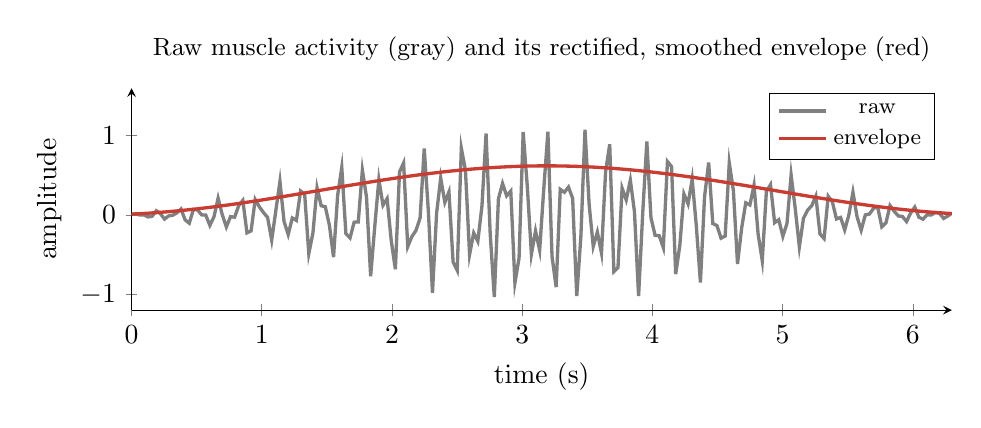
\begin{tikzpicture}
\begin{axis}[
title style={font=\small},
    width=12cm, height=4.4cm,
    xlabel={time (s)}, ylabel={amplitude},
    xmin=0, xmax=6.3, ymin=-1.2, ymax=1.6,
    axis lines=left, samples=200, domain=0:6.3,
    title={Raw muscle activity (gray) and its rectified, smoothed envelope (red)},
    every axis plot/.append style={line width=0.8pt},
    legend style={font=\footnotesize, at={(0.98,0.98)}, anchor=north east},
]
\addplot[gray, very thick] {(0.5+0.5*sin(deg(0.9*x-1.3)))*(0.7*sin(deg(40*x))+0.5*sin(deg(67*x+1)))};
\addlegendentry{raw}
\addplot[specred, very thick] {0.62*(0.5+0.5*sin(deg(0.9*x-1.3)))};
\addlegendentry{envelope}
\end{axis}
\end{tikzpicture}
\caption{The key de-noising move for FMG/sEMG. The raw signal (gray) is a fast
oscillation gated on and off as the muscle contracts. We do not care about the
oscillation, only \emph{that it is present and how strong}. Full-wave rectifying
($\abs{x}$) and low-pass smoothing extracts the envelope (red) --- a slow signal
whose height is a clean proxy for contraction strength.}
\label{ch41:fig-emgenv}
\end{figure}

The recipe, stream by stream:

\begin{enumerate}
  \item \textbf{sEMG:} bandpass $20$--$450\,$Hz (remove DC drift and out-of-band
        junk), notch at $50$ or $60\,$Hz (mains), then \emph{rectify}
        ($\abs{x}$ or $x^2$) and \emph{low-pass} at a few hertz to get the
        linear envelope. The rectify-then-smooth pair is exactly the
        magnitude-then-average idea from the analytic-signal chapter; it converts
        ``how much muscle drive'' into a slow controllable number.
  \item \textbf{FMG:} the FSR voltage already \emph{is} a slow envelope, so just
        low-pass it (a one-pole smoother or short moving average, Chapter~17) to
        kill ADC jitter and the odd spike. No rectification needed --- pressure
        is one-sided.
  \item \textbf{IMU:} a light low-pass on the accelerometer (remove vibration
        hash) and a gyro-bias estimate at rest; then hand both to the fusion
        filter. Do \emph{not} aggressively low-pass the gyro --- you would add
        lag to your orientation, which the player feels.
\end{enumerate}

\begin{whybox}
Why rectify and smooth instead of, say, taking the spectrum? Because the
\emph{information you want is in the amplitude, not the waveform}. A contracting
muscle produces a roughly stochastic burst whose exact zero-crossings are
meaningless; what carries the gesture is the burst's \emph{strength and which
channels light up}. Rectify-and-smooth is the cheapest unbiased estimator of
that strength --- it is the matched move for an amplitude-modulated random
carrier, and it runs in a handful of operations per sample, which matters when
you are on a microcontroller meeting a deadline.
\end{whybox}

\section{Calibration: the heart of the instrument}
\label{ch41:calibration}

This is the section that makes the whole thing work without machine learning. No
two arms, and no two strap-ons of the \emph{same} arm, give the same raw numbers.
Calibration (Chapter~35) makes the device work for a real person on a real
morning rather than only on the bench where you tuned it --- and, done as a
\emph{per-finger enrollment}, it is also what lets a direct match identify which
finger moved.

\subsection{Step one: per-channel baseline and scale}

Before any finger means anything, put the channels on a common footing. At the
start of a session, ask the user to rest the hand for one second; record each
channel's mean, the \emph{rest baseline} $b_i$. Then ask for one maximum
voluntary contraction (a hard fist) for a second and record each channel's peak
$p_i$. Normalize every later sample to
\[
  \tilde{x}_i[n] \;=\; \frac{x_i[n] - b_i}{p_i - b_i},
\]
so each channel lands in roughly $[0,1]$ regardless of skin, strap tension, or
electrode contact. This single affine fix removes most cross-session variation.

\subsection{Step two: per-finger enrollment and templates}
\label{ch41:enroll}

Now the part that replaces a learned model. The phone runs a short, guided
\emph{enrollment}: it names a finger movement, the user performs it a few times,
and the phone records the resulting normalized sensor pattern. There is no
training of weights and no optimizer --- just recording and averaging.

\begin{enumerate}
  \item For each movement $g$ in the vocabulary (rest, index, middle, ring,
        little, fist, spread, \ldots), the phone prompts ``move your index
        finger,'' and the user repeats it, say, five times.
  \item For each repetition the phone computes the per-frame feature vector
        (Section~\ref{ch41:features}) at the moment of peak activity --- the
        normalized envelope across all FMG, sEMG, and contact channels.
  \item It \emph{averages} those repetitions into one prototype vector, the
        \textbf{template} $\vec{t}_g$, and records the spread (a per-channel
        standard deviation) so it knows how tight each finger's signature is.
\end{enumerate}

The result is a tiny table: one template vector per finger movement, plus a
spread. That table \emph{is} the user's personalized model. It takes under a
minute to build, lives in a few hundred bytes, and is pushed down to the wrist
node so live matching needs no phone.

\begin{figure}[H]
\centering
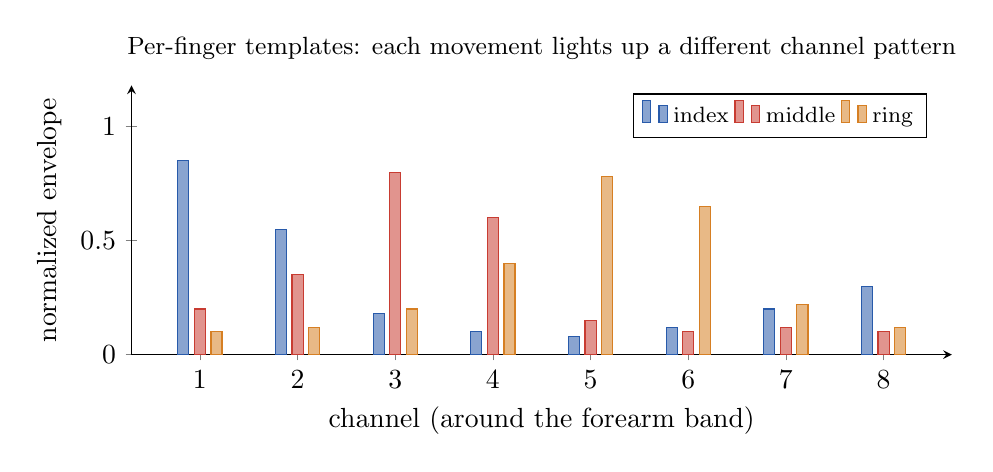
\begin{tikzpicture}
\begin{axis}[
title style={font=\small},
    width=12cm, height=5cm,
    ybar, bar width=4pt,
    xlabel={channel (around the forearm band)}, ylabel={normalized envelope},
    xmin=0.3, xmax=8.7, ymin=0, ymax=1.18,
    xtick={1,2,3,4,5,6,7,8},
    axis lines=left,
    title={Per-finger templates: each movement lights up a different channel pattern},
    legend pos=north east, legend style={font=\footnotesize, legend columns=3},
]
\addplot[draw=sigblue, fill=sigblue!55] coordinates {(1,0.85)(2,0.55)(3,0.18)(4,0.10)(5,0.08)(6,0.12)(7,0.20)(8,0.30)};
\addlegendentry{index}
\addplot[draw=specred, fill=specred!55] coordinates {(1,0.20)(2,0.35)(3,0.80)(4,0.60)(5,0.15)(6,0.10)(7,0.12)(8,0.10)};
\addlegendentry{middle}
\addplot[draw=quotientorange, fill=quotientorange!55] coordinates {(1,0.10)(2,0.12)(3,0.20)(4,0.40)(5,0.78)(6,0.65)(7,0.22)(8,0.12)};
\addlegendentry{ring}
\end{axis}
\end{tikzpicture}
\caption{Three enrolled templates over an 8-channel FMG band. Each finger
movement bulges a different group of forearm muscles, so it raises a different
\emph{spatial} pattern of normalized envelopes. Live detection compares the
current 8-vector to these prototypes and picks the nearest. The patterns overlap
in places --- ring and middle share channel 4 here --- which is why the extra
sEMG and contact channels, and a tight calibration, matter.}
\label{ch41:fig-templates}
\end{figure}

\subsection{Step three: IMU calibration}

Gyros have a slowly-drifting bias: average a couple of seconds at rest and
subtract it (re-estimate whenever the device is still). Accelerometers need the
standard offset-and-scale-per-axis fit from Chapter~35 so that ``1\,g down''
reads as exactly $1\,g$; otherwise your gravity-derived tilt, and thus your
pitch-to-note mapping, is skewed.

\begin{connectionbox}
The normalization in step one is the affine \emph{whitening} you met in the
linear algebra companion: subtract a mean, divide by a scale, to put every
coordinate on comparable footing before measuring distances. Template matching
compares feature vectors by distance, which implicitly assumes the axes are
commensurate --- calibration is what makes that assumption true. Skip it and a
single dominant channel swamps the distance metric. The per-finger templates of
step two then place one labelled landmark per movement in that whitened space,
and detection is simply ``which landmark is nearest.''
\end{connectionbox}

\section{Windowing and feature extraction}
\label{ch41:features}

The matcher does not eat raw samples; it eats \emph{feature vectors} computed
over a short window. This is the short-time idea from Chapter~10: slice the
stream into overlapping frames and summarize each frame with a few numbers. The
same feature vector is computed during enrollment (to build templates) and during
play (to match them), so the two stay comparable by construction.

\paragraph{Frame geometry.} Use a window of $W = 128$--$256\,$ms with
$50$--$75\,\%$ overlap, recomputed every \emph{hop} of $\sim$\,$32\,$ms. A
shorter window means lower latency but noisier features; a longer window is
steadier but laggier. For a played instrument, $W \approx 150\,$ms with a
$30\,$ms hop is a good corner of that trade-off --- it updates the finger
decision about $30$ times a second, which feels instantaneous.

\paragraph{Features that work for muscle sensors.} The literature (and a lot of
hard-won practice) converges on cheap \emph{time-domain} features per channel,
because they are robust and microcontroller-friendly:

\begin{itemize}
  \item \textbf{Mean absolute value (MAV):}
        $\frac{1}{W}\sum_n \abs{x_i[n]}$ --- the envelope height; the single
        most useful feature.
  \item \textbf{Root mean square (RMS):}
        $\sqrt{\frac{1}{W}\sum_n x_i^2[n]}$ --- energy; closely related to
        perceived contraction strength.
  \item \textbf{Waveform length:} $\sum_n \abs{x_i[n]-x_i[n-1]}$ --- captures
        signal complexity/activity cheaply.
  \item \textbf{Zero crossings} and \textbf{slope-sign changes:} crude frequency
        proxies for sEMG; usually skip for slow FMG.
\end{itemize}

A handful of spectral features can help sEMG --- the \emph{mean} and
\emph{median frequency} of the power spectrum shift as a muscle fatigues, and a
short FFT (Chapter~9) gives them for nearly free --- but for a first build the
time-domain features above carry most of the discriminating power.

\begin{focusbox}
The \emph{spatial} pattern across channels is where the finger lives. A single
channel's MAV tells you ``some muscle fired''; the \emph{vector} of MAVs across
all channels tells you \emph{which} muscles and thus \emph{which} finger moved.
For an 8-channel band the per-frame feature vector might be just the 8 MAVs plus
8 waveform-lengths --- a 16-dimensional point. Detection is then: which enrolled
template is this point closest to?
\end{focusbox}

\begin{lstlisting}[language=Python]
import numpy as np

def frame_features(frame):
    """frame: shape (W, C), one window of C channels. Returns 1D feature vector."""
    x   = frame.astype(np.float32)
    mav = np.mean(np.abs(x), axis=0)                 # (C,) envelope height
    rms = np.sqrt(np.mean(x*x, axis=0))              # (C,) energy
    wl  = np.sum(np.abs(np.diff(x, axis=0)), axis=0) # (C,) waveform length
    return np.concatenate([mav, rms, wl])            # (3C,)
\end{lstlisting}

\subsection{Why a small feature set beats raw samples}

\begin{happeningbox}
A $150\,$ms window at $1\,$kHz across 8 channels is $1200$ raw numbers per
frame. The 16 (or 24) features above compress that by nearly a hundredfold while
\emph{keeping} what separates the fingers and \emph{throwing away} the stochastic
detail that only muddies a match. This is dimensionality reduction in the service
of separability: you are projecting a noisy high-dimensional frame onto the few
directions that actually move between fingers. Matching then works in a space
small enough to describe with one template per finger and fast enough to evaluate
every hop on a microcontroller.
\end{happeningbox}

\section{Template matching: detection without a learned model}
\label{ch41:matching}

We have, per frame, a low-dimensional feature vector $\vec{x}$, and from
enrollment (Section~\ref{ch41:enroll}) one template vector $\vec{t}_g$ per finger
movement. Detection is now embarrassingly direct: which template is the current
frame closest to?
\[
  \hat{g}[n] \;=\; \arg\min_{g}\; \norm{\vec{x}[n] - \vec{t}_g}^2 .
\]
That is the whole decision rule. No weights are fit, no optimizer runs, no
network is trained --- the only ``model'' is the table of per-user templates the
phone recorded in under a minute. This is nearest-template matching, and it is
the geometry of Chapter~39's inner product put to work: the squared distance
$\norm{\vec{x}-\vec{t}_g}^2 = \norm{\vec{x}}^2 - 2\inner{\vec{x}}{\vec{t}_g} +
\norm{\vec{t}_g}^2$ is small exactly when the frame \emph{correlates} strongly
with the finger's signature.

\paragraph{Distance or correlation.} For amplitude-stable, calibrated channels,
Euclidean distance to the template is the natural rule. If overall contraction
\emph{strength} varies but the \emph{pattern} is what identifies the finger, use
the normalized correlation (cosine similarity) instead,
\[
  s_g[n] \;=\; \frac{\inner{\vec{x}[n]}{\vec{t}_g}}
                    {\norm{\vec{x}[n]}\,\norm{\vec{t}_g}},
\]
and pick the largest. Cosine matching shrugs off a global ``pressed harder this
time'' scaling, which the distance rule would penalize.

\paragraph{Reject when nothing matches.} The \textbf{rest} template handles the
common ``no finger moved'' case as a first-class entry --- without it the matcher
would always snap to the nearest \emph{active} finger and hallucinate notes. Add
a guard too: if even the best distance exceeds a threshold (the live frame is far
from every template), declare rest rather than force a match. The per-finger
spread recorded during enrollment sets that threshold per movement.

\begin{figure}[H]
\centering
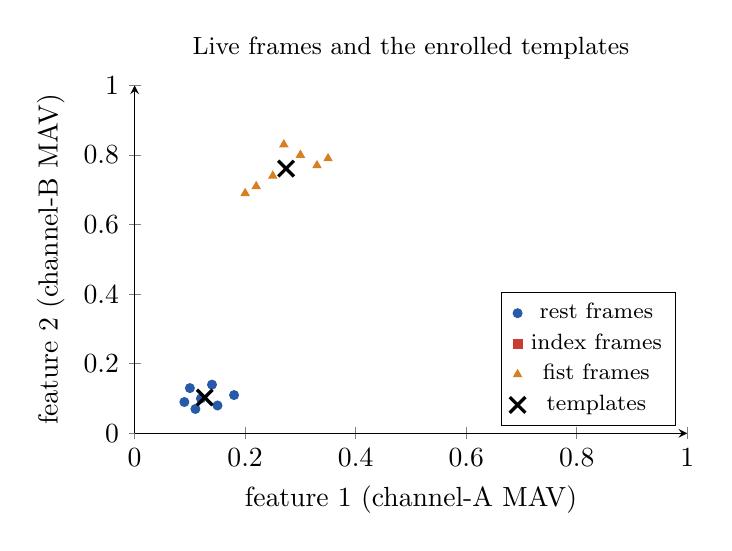
\begin{tikzpicture}
\begin{axis}[
title style={font=\small},
    width=8.6cm, height=6.0cm,
    xlabel={feature 1 (channel-A MAV)}, ylabel={feature 2 (channel-B MAV)},
    xmin=0, xmax=1, ymin=0, ymax=1,
    axis lines=left,
    title={Live frames and the enrolled templates},
    legend style={font=\footnotesize, at={(0.98,0.02)}, anchor=south east},
    mark size=1.6pt,
]
\addplot[sigblue, only marks, mark=*] coordinates {
 (0.12,0.10)(0.15,0.08)(0.10,0.13)(0.18,0.11)(0.09,0.09)(0.14,0.14)(0.11,0.07)};
\addlegendentry{rest frames}
\addplot[specred, only marks, mark=square*] coordinates {
 (0.72,0.20)(0.78,0.24)(0.69,0.18)(0.81,0.22)(0.74,0.27)(0.70,0.15)(0.83,0.25)};
\addlegendentry{index frames}
\addplot[quotientorange, only marks, mark=triangle*] coordinates {
 (0.25,0.74)(0.30,0.80)(0.22,0.71)(0.33,0.77)(0.27,0.83)(0.20,0.69)(0.35,0.79)};
\addlegendentry{fist frames}
\addplot[black, only marks, mark=x, mark size=4pt, line width=1.2pt] coordinates {
 (0.127,0.103)(0.752,0.216)(0.274,0.761)};
\addlegendentry{templates}
\end{axis}
\end{tikzpicture}
\caption{Why nearest-template matching suffices. Projected onto two channel MAVs,
each finger movement's live frames form a tight cloud, and the enrolled template
($\times$) is just their average. A new frame is labelled by the nearest
$\times$. Calibration put each channel in $[0,1]$, which makes the clouds compact
and the distances meaningful; the extra sEMG and contact channels separate clouds
that would overlap in these two FMG dimensions alone.}
\label{ch41:fig-clusters}
\end{figure}

\begin{lstlisting}[language=Python]
import numpy as np
# templates: (G, D) one row per finger movement (incl. "rest"); built at enrollment
# reject_dist: per-template distance threshold from the enrollment spread

def detect(x, templates, labels, reject_dist):
    d = np.sum((templates - x)**2, axis=1)   # squared distance to each template
    g = int(np.argmin(d))
    if d[g] > reject_dist[g]:                # too far from everything -> rest
        return "rest"
    return labels[g]
\end{lstlisting}

A handful of multiplies and adds per template, a few templates: this runs in
microseconds on the wrist node, which is exactly why the live path does not need
the phone.

\begin{trapbox}
\textbf{Check generalization on a fresh strap-on, not the enrollment run.} It is
tempting to declare victory because the enrolled frames match their own
templates --- of course they do, the templates are their average. The real test
is re-donning the band and matching against the existing templates without
re-enrolling. The day you re-don the band is the day you discover how much the
signatures depend on exact placement. If accuracy sags, that is the cue to add a
quick 3-second recalibration ritual on each don (Section~\ref{ch41:recal}),
not to reach for a bigger model.
\end{trapbox}

\subsection{Smoothing the decision: from frame labels to finger events}
\label{ch41:statemachine}

A per-frame match flickers --- one stray frame mid-movement matches ``fist'' for
$30\,$ms. Raw, that becomes a spurious MIDI note. Tame it with a small
\emph{state machine} and \emph{debouncing}, exactly the hysteresis idea from the
practical-filtering chapter:

\begin{itemize}
  \item Require $N$ consecutive frames (e.g.\ 3) agreeing before declaring a new
        finger event (majority vote over a short sliding window).
  \item Require a return to \textbf{rest} before the same movement can fire again
        --- this gives you crisp note \emph{onsets} instead of a stuttering
        retrigger.
  \item Confidence-gate: if the best match is barely closer than the runner-up
        (small margin), hold the previous state rather than switch.
\end{itemize}

\begin{figure}[H]
\centering
\begin{tikzpicture}[
    font=\small, >=Latex,
    st/.style={draw, circle, minimum size=11mm, align=center},
]
\node[st, fill=blue!6] (rest) {rest};
\node[st, fill=green!8, right=24mm of rest] (armed) {armed\\($k{<}N$)};
\node[st, fill=violet!10, right=24mm of armed] (fire) {firing\\(Note On)};
\draw[->] (rest) to[bend left=18] node[above, font=\footnotesize]{match $g$} (armed);
\draw[->] (armed) to[bend left=18] node[below, font=\footnotesize]{not $g$} (rest);
\draw[->] (armed) to[bend left=18] node[above, font=\footnotesize]{$N$ agree} (fire);
\draw[->] (fire) to[bend left=30] node[below, font=\footnotesize]{back to rest $\Rightarrow$ Note Off} (rest);
\end{tikzpicture}
\caption{The debouncing state machine. A candidate match must survive $N$ frames
in the \emph{armed} state before it fires a Note On; the same movement cannot
fire again until the hand passes back through \emph{rest}, which is also when the
Note Off is sent. This turns a flickering per-frame label stream into crisp,
non-repeating note events.}
\label{ch41:fig-statemachine}
\end{figure}

\section{Sensor fusion: the IMU as the expressive axis}
\label{ch41:fusion}

While the muscle branch decides \emph{what}, the IMU branch decides \emph{how}.
From Chapter~36 we fuse accelerometer (good long-term tilt reference from
gravity, noisy short-term) and gyroscope (clean short-term rotation rate, drifts
long-term) into a stable orientation --- a complementary filter is enough:
\[
  \theta[n] \;=\; \alpha\,\bigl(\theta[n-1] + \omega_{\text{gyro}}[n]\,T_s\bigr)
              \;+\; (1-\alpha)\,\theta_{\text{accel}}[n],
\]
with $\alpha$ near $0.98$. The gyro term gives responsiveness; the small accel
term slowly pulls out drift. Out of this you get wrist \emph{pitch} and
\emph{roll} (yaw needs a magnetometer and is the least reliable --- avoid making
it musically load-bearing).

\begin{goalbox}
Map the fused orientation to expression:
\begin{itemize}
  \item \textbf{Wrist pitch} $\to$ pitch bend or note selection (tilt up to go
        sharp).
  \item \textbf{Wrist roll} $\to$ a continuous controller (CC 1, modulation /
        vibrato depth).
  \item \textbf{Motion energy} (gyro magnitude) $\to$ note velocity or CC 11
        (expression): a fast, snappy gesture hits harder than a lazy one.
\end{itemize}
These are \emph{continuous} and feel alive precisely because the IMU genuinely
measures them well --- the opposite of trying (and failing) to read finger
angles from the same sensor.
\end{goalbox}

\section{Latency budgeting}
\label{ch41:latency}

A musical controller lives or dies on latency. The well-known threshold for
``feels instantaneous'' on a played instrument is about $10\,$ms; up to
$\sim$\,$20$--$30\,$ms is usable; beyond that you feel the rubber band. Every
stage in Figure~\ref{ch41:fig-pipeline} spends some of that budget. Add them up
without flinching.

\begin{historybox}
In 2002, David Wessel and Matthew Wright published their landmark paper \emph{``Problems and Prospects for Intimate Musical Control of Computers''} (Computer Music Journal, UC Berkeley CNMAT). They asked a fundamental question: \emph{why do digital and gesture-based electronic instruments feel so disconnected and emotionally cold compared to an acoustic cello, trumpet, or drum?}

The answer was temporal immediacy and tactile feedback. In an acoustic instrument, mechanical vibrations propagate from finger or bow to sounding body in microseconds; total acoustic latency from physical strike to ear is under $1$ to $5\,\text{ms}$. Wessel and Wright experimentally mapped human perceptual thresholds for musical control. Below $10\,\text{ms}$, the player experiences \emph{instantaneous intimacy}: the sonic response feels directly coupled to bodily action, and haptic bone conduction, muscle contraction, and audio fuse into a unified tactile sensation. Between $10$ and $20\,\text{ms}$, latency becomes perceptible though playable: skilled musicians can compensate for steady delay by anticipation, though fast rhythmic passages (such as $16\text{th}$-note drum rolls at $140$~BPM, where notes are separated by only $107\,\text{ms}$) begin to feel sluggish. Above $30\,\text{ms}$, the illusion of physical causality collapses: the human motor-control loop perceives the sound as an external echo rather than an extension of the limb, and rhythmic synchronization disintegrates into jitter. To build an intimate wearable instrument, every microsecond along the chain---from muscle fiber contraction to audio speaker cone---must be ruthlessly budgeted.
\end{historybox}

\begin{table}[H]
\centering
\small
\begin{tabular}{@{}llr@{}}
\toprule
Stage & Mechanism \& Constraint & Typical Latency \\
\midrule
Transducer \& Acoustic & Muscle mechanical bulge / skin wave propagation & $1$--$2\,$ms \\
Analog Front-End & Anti-alias $RC$ filter group delay & $1$--$2\,$ms \\
ADC \& Conditioning & Multi-channel SAADC conversion + 60\,Hz notch group delay & $2$--$4\,$ms \\
Envelope \& Smoothing & One-pole / IIR low-pass smoothing filter group delay & $4$--$8\,$ms \\
Window \& Matching & 150\,ms window with 30\,ms hop + 2-frame debounce & $15$--$30\,$ms \\
BLE 5.0 Wireless & BLE Connection Interval (Nordic SoftDevice min 7.5\,ms) + radio queue & $7.5$--$15\,$ms \\
Host Audio Buffer & DAW / Synth driver buffer (128 samples @ 48\,kHz) & $2.7$--$5.3\,$ms \\
\midrule
\textbf{Total End-to-End} & \textbf{Realistic physical-strike to acoustic emission} & \textbf{$\approx$ 33--66\,ms} \\
\bottomrule
\end{tabular}
\caption{The end-to-end latency budget from physiological intention to acoustic output. The major bottlenecks are the digital feature window/debounce and the wireless BLE connection interval. Shaving latency requires streaming sparse events and tuning filter cutoffs to the specific articulation.}
\label{ch41:tab-latency-breakdown}
\end{table}

\begin{focusbox}
The latency triangle from Chapter~17 reappears here in disguise: \emph{quality}
(clean envelope, a confident match) costs \emph{latency} (longer window,
slower LPF, more debounce frames). For a forgiving sustained-pad sound you can
spend latency freely; for a percussive, snappy lead you must shrink the window,
loosen the debounce, and accept more flicker. Tune the budget \emph{to the
sound}, not to a universal number.
\end{focusbox}

\begin{trapbox}
The sneakiest latency is the one you forget: the synth/DAW's own audio buffer.
A $512$-sample buffer at $48\,$kHz is already $\sim$\,$11\,$ms before your MIDI
even becomes sound. Measure end-to-end (tap the band, record the audio,
count samples to the attack) rather than trusting the sum of your estimates.
\end{trapbox}

\section{MIDI mapping}
\label{ch41:midi}

The final box turns gesture state and orientation into MIDI bytes. The mapping
\emph{is} the instrument design --- the same hardware feels utterly different
under different maps.

\begin{historybox}
In the late 1990s and early 2000s, early digital instrument designers fell into an enticing but disastrous trap: naive one-to-one mapping. If an IMU measures pitch angle, why not wire pitch angle directly to synthesizer frequency? If roll measures angle, why not wire it to volume?

As Andy Hunt and Ross Kirk (2000, University of York) and Marcelo Wanderley (2002, McGill / IRCAM) proved through extensive user studies, one-to-one mapping produces an unplayable caricature of an instrument---an uncontrollable ``arm Theremin.'' If every microscopic tremor or arm repositioning shifts the fundamental frequency, the musician cannot play a stable pitch while gesturing to a bandmate or adjusting their posture.

Wanderley and Hunt formalized the taxonomy of musical mapping: whereas a fragile \emph{one-to-one} mapping ties one sensor variable to one acoustic parameter ($\theta \to f_0$), an expressive acoustic instrument uses \emph{one-to-many} (divergent) mappings where a single gestural action simultaneously modulates multiple acoustic timbres (striking faster increases volume, brightens the cutoff frequency, and shortens envelope decay) and \emph{many-to-one} (convergent) mappings where multiple sensor streams collaboratively determine a musical state (FMG muscle flexion gates the note onset while fused IMU attitude and angular velocity modulate pitch vibrato and timbre). The wristband controller succeeds precisely because it decouples discrete gating (finger flexors recruit specific notes) from continuous spatial modulation (wrist attitude shapes timbre and vibrato).
\end{historybox}

\begin{trapbox}
\textbf{The Fatal BLE Transport Trap: Streaming Raw Waves vs Sparse Event Extraction}

A naive firmware architecture for a wireless wearable tries to stream raw multi-channel sensor samples over Bluetooth Low Energy (BLE) to a host computer for processing. Consider the bandwidth arithmetic:
\begin{itemize}
  \item 8 channels of 12-bit FMG at $100\,$Hz = $9.6\,$kbps
  \item 1 channel of 12-bit sEMG at $1000\,$Hz = $12.0\,$kbps
  \item 6 axes of 16-bit IMU (accel + gyro) at $200\,$Hz = $19.2\,$kbps
  \item 1 high-rate contact accelerometer at $4000\,$Hz = $48.0\,$kbps
\end{itemize}
Including GATT protocol framing and packet headers, the continuous throughput exceeds $120\,$kbps. Under BLE 4.2/5.0 GATT notification limits, streaming continuous high-rate waveforms chokes the Nordic SoftDevice radio FIFO queues. Packets are dropped, transmission latency unpredictably spikes from $10\,$ms to over $200\,$ms during RF interference, and the radio transmitter must remain active at 100\% duty cycle, draining a $150\,\text{mAh}$ coin cell or LiPo battery in under 2 hours!

\textbf{The Solution: Edge Extraction.} Run the filtering, Madgwick attitude fusion, and template matching directly on the nRF52840's ARM Cortex-M4F core. Transmit \emph{only} 3-byte MIDI events on gesture triggers (\texttt{0x90} Note-On, \texttt{0x80} Note-Off) and decimated $50\,$Hz orientation updates as 4-byte packed Pitch-Bend / CC messages. Total wireless data rate plummets to under $1.5\,$kbps ($>95\%$ reduction), latency drops to a rock-solid single connection interval ($7.5\,$ms), and battery life extends beyond 24 continuous hours.
\end{trapbox}

\paragraph{Notes from gestures.} On a confirmed gesture onset, send
\texttt{Note On} (status \texttt{0x90}, note number, velocity); on the return to
rest, send \texttt{Note Off} (\texttt{0x80}). Derive the note number from the
gesture identity (index pinch $\to$ scale degree 1, middle pinch $\to$ degree 3,
\ldots) or from wrist pitch quantized to a scale. Derive velocity from motion
energy at onset.

\paragraph{Chords.} Map a gesture to a \emph{set} of simultaneous Note Ons ---
``fist'' could strike a triad. Honor the gesture vocabulary's discreteness here
rather than fighting it; chords are a natural fit for a small, reliable gesture
set.

\paragraph{Continuous control.} Stream wrist roll as CC 1 (mod wheel) and pitch
as Pitch Bend (14-bit, status \texttt{0xE0}) \emph{between} note events. Smooth
and rate-limit these (send at most every few ms) so you do not flood the bus.

\begin{lstlisting}[language=Python]
import mido
port = mido.open_output()                       # a virtual MIDI port into your DAW

def on_gesture(gesture, velocity, channel=0):
    note = GESTURE_TO_NOTE[gesture]             # e.g. {"index_pinch": 60, ...}
    port.send(mido.Message('note_on', note=note, velocity=velocity, channel=channel))

def on_release(gesture, channel=0):
    note = GESTURE_TO_NOTE[gesture]
    port.send(mido.Message('note_off', note=note, channel=channel))

def on_orientation(roll, pitch_bend, channel=0):
    cc = int(max(0, min(127, roll * 127)))      # roll in [0,1] -> CC1
    port.send(mido.Message('control_change', control=1, value=cc, channel=channel))
    pb = int(max(-8192, min(8191, pitch_bend)))
    port.send(mido.Message('pitchwheel', pitch=pb, channel=channel))
\end{lstlisting}

\begin{applicationbox}
The same controller, three instruments, just by swapping the map:
\begin{itemize}
  \item \textbf{Lead synth:} gestures pick scale degrees, wrist pitch bends,
        roll adds vibrato --- an expressive monophonic solo voice.
  \item \textbf{Chord pad:} each gesture is a chord; motion energy sets
        velocity; roll opens a filter via CC --- a one-hand harmony rig.
  \item \textbf{Drum trigger:} each gesture is a drum (kick, snare, hat);
        velocity from snap strength --- finger-drumming in the air.
\end{itemize}
Nothing about the signal chain changed; only \texttt{GESTURE\_TO\_NOTE} and the
CC routing did. That is the leverage of clean separation between sensing and
mapping.
\end{applicationbox}

\section{Bill of materials}
\label{ch41:bom}

\begin{table}[H]
\centering
\small
\begin{tabular}{@{}llr@{}}
\toprule
Item & Notes & Rough cost \\
\midrule
Microcontroller (Teensy 4.x / RP2040 / ESP32) & USB-MIDI capable, $\ge 8$ ADC ch & \$10--\$30 \\
8$\times$ FSR (Interlink 402 or similar) & FMG sensing band & \$25--\$40 \\
8$\times$ 10\,k$\Omega$ resistors & divider legs & \$1 \\
IMU breakout (MPU-6050 / ICM-20948 / BMI270) & accel + gyro ($+$ mag opt.) & \$5--\$15 \\
Elastic strap + hook-loop & forearm band & \$5 \\
Wire, perfboard/flex PCB, connectors & assembly & \$10 \\
\midrule
\textbf{FMG build total} & & \textbf{$\sim$\,\$60--\$100} \\
\midrule
\emph{Alt: sEMG path} MyoWare 2.0 ($\times 1$--$3$) or used Myo & adds gel/electrodes & +\$40--\$150 \\
\bottomrule
\end{tabular}
\caption{A realistic bill of materials. The FMG path is deliberately the cheap,
forgiving entry point; sEMG is an optional accuracy/latency upgrade at real
cost and difficulty.}
\label{ch41:tab-bom}
\end{table}

\section{Accuracy, difficulty, and failure modes}
\label{ch41:recal}

\begin{trapbox}
\textbf{Accuracy and difficulty, told straight.}
\begin{itemize}
  \item A \textbf{5--6 finger-movement} vocabulary, well calibrated, on the
        \emph{same} session realistically hits $\sim$\,$85$--$95\,\%$ per-frame
        accuracy --- excellent for music, where the state machine cleans up
        stragglers. WristFlex reported around $80\,\%$ from FMG alone; the extra
        sEMG and contact channels here push that up, which is the point of going
        multimodal.
  \item Accuracy \textbf{drops} when you re-don the band, when you sweat, when
        your arm posture changes, and as the movement count grows. Cross-session,
        un-recalibrated accuracy can fall 10--20 points. Re-running the 30-second
        per-finger enrollment on each don recovers it --- which is why
        calibration, not a model, is the thing you maintain.
  \item \textbf{Distinguishing adjacent fingers} (index vs.\ ring, say) is the
        hard end of the achievable range. FMG alone can blur them where their
        muscle bulges overlap; the sEMG channel and the contact-onset timing are
        exactly what pull the templates apart. Enroll those pairs with extra care
        and keep them spatially distinct in your mapping.
  \item \textbf{Continuous per-joint finger angles: not from this hardware.} This
        is the genuinely underdetermined part --- see
        Section~\ref{ch41:upgrade}. Everything a player needs (which finger,
        how hard, wrist shaping) sits on the achievable side.
\end{itemize}
\end{trapbox}

Failure modes you \emph{will} meet, and the fix for each:

\begin{itemize}
  \item \textbf{Band shifts during play} $\to$ pressure pattern changes, matches
        misfire. Fix: snug strap, repeatable placement marks, quick re-enroll.
  \item \textbf{Mains hum (sEMG)} $\to$ $50/60\,$Hz buzz dominates. Fix: notch
        filter, shorter electrode leads, battery (not USB-wall) power, move away
        from the laptop charger.
  \item \textbf{Motion artifact} $\to$ a vigorous arm move slams the envelope and
        triggers a phantom note. Fix: gate the matcher with the IMU --- if gross
        arm motion is high, raise the match-distance threshold.
  \item \textbf{Drift / fatigue (sEMG)} $\to$ envelope baseline creeps over
        minutes. Fix: slow adaptive baseline (track and subtract a long-term
        mean per channel), which keeps the templates valid without re-enrolling.
  \item \textbf{Note stutter} $\to$ match flicker. Fix: the state-machine
        debounce of Section~\ref{ch41:statemachine}.
  \item \textbf{Stuck notes} $\to$ a missed Note Off. Fix: a watchdog that sends
        \texttt{All Notes Off} (CC 123) on any unexpected state, and on rest.
\end{itemize}

\begin{labbox}
Before wiring anything, prototype the \emph{whole} pipeline in software on a
recorded log: capture a few minutes of multi-channel FMG (or a public sEMG
dataset), then run conditioning $\to$ features $\to$ enroll templates $\to$
nearest-template match $\to$ a printed finger label, offline. You will shake out
most of the bugs without a soldering iron, and you will have a labelled dataset
ready for the real-time port.
\end{labbox}

\section{Upgrade path}
\label{ch41:upgrade}

When the finger controller delights you and you want \emph{more}, here is the
ladder --- each rung adds real capability at real cost, and only the last one
crosses into the genuinely hard territory.

\begin{enumerate}
  \item \textbf{More sEMG channels} (8+ around the forearm) $\to$ larger, finer
        movement vocabularies and crisper templates for adjacent fingers; the
        Myo/MyoWare territory and the MDPI Sensors fusion benchmarks.
  \item \textbf{Richer contact sensing} (a dedicated high-rate accelerometer or
        contact mic, ViBand-style) $\to$ sharper tap, scratch, and surface-contact
        detection for percussive triggers, beyond what the shared IMU catches.
  \item \textbf{Finger-ring inertial sensors} $\to$ the route to \emph{continuous
        individual finger pose}, the one thing the wrist genuinely cannot give.
        Put a tiny IMU on each finger (``Learning on the Rings''); now you measure
        each finger's motion directly instead of inferring it from the forearm.
        This is the real glove-replacement, and it is fundamentally a
        \emph{different sensor placement}, not a smarter wrist algorithm. It is an
        upgrade, not a requirement: the wrist band already plays.
\end{enumerate}

\begin{aestheticbox}
Notice what the whole book bought you. Sampling and Nyquist set the rates;
anti-alias and notch filtering cleaned the streams; rectify-and-smooth (the
analytic-signal envelope) made amplitude readable; windowing and the FFT (the
short-time view) framed the features; inner-product geometry made nearest-template
matching intelligible; complementary fusion turned two flawed motion sensors into
one good orientation; per-finger calibration replaced a learned model with a
table you build in under a minute; and the latency triangle disciplined every
choice. The finger controller is not a new subject --- it is every chapter,
wearing a strap.
\end{aestheticbox}

\section{Capabilities, Limitations, and the Road Ahead}
\label{ch41:capabilities-road-ahead}

\subsection{What the Wristband Gesture Controller Unlocked}

Building the wrist-worn gesture controller brings together every strand of signal processing developed in this book into a unified cybernetic instrument:
\begin{itemize}
  \item \textbf{Camera-Free Non-Invasive Expressive Control:} Optical vision systems (such as Leap Motion or Kinect) suffer from field-of-view limits, line-of-sight occlusion when hands turn or cross, and variable room lighting. Mechanical data gloves restrict tactile sensation and require bulky, fragile exoskeletons. The wristband sits entirely on the arm, leaving the hands and fingers free to touch real instruments, keyboards, or open air anywhere on stage.
  \item \textbf{Calibration Beats Brute-Force Modeling:} By replacing brittle, multi-thousand-weight deep neural networks with deterministic physical filtering, Madgwick quaternion integration, and a 60-second guided template enrollment, the instrument runs on a micro-power microcontroller with zero training infrastructure and zero black-box unpredictability.
  \item \textbf{Multimodal Synergy:} Fusing muscle mechanics (FMG for steady finger posture), electrophysiology (sEMG for explosive onset timing), bio-acoustics (high-rate accelerometer for transient contact spikes), and inertial dynamics (IMU for spatial orientation) yields a holistic sensing interface where the strengths of each physical domain cancel the blind spots of the others.
\end{itemize}

\subsection{Honest Downsides and Physical Limitations}

An engineer must never confuse a working laboratory prototype with an unconstrained magic wand. Wearable bio-signal processing faces severe physical constraints:
\begin{itemize}
  \item \textbf{Inertial-Muscular Mechanical Cross-Talk:} When a performer swings their arm violently across the stage, centripetal acceleration and inertia tug on the forearm muscles, displacing the strap and shifting sensor-to-skin pressure. This gross body movement produces spurious FMG pressure fluctuations and sEMG movement artifacts that can mimic a finger contraction or corrupt enrolled templates.
  \item \textbf{The Underdetermined Finger Pose Barrier:} Tendons in the forearm branch and slide over one another in a dense mechanical sheath (the carpal tunnel). As established in Section~\ref{ch41:goal}, recovering the continuous $20$-degree-of-freedom joint angles of five independent fingers from a surface wristband is mathematically ill-posed. Discrete finger triggers work reliably; continuous virtual piano playing without finger-worn sensors remains beyond reach.
  \item \textbf{Sweat, Fatigue, and Electrode Impedance Drift:} Over extended performances, perspiration changes skin conductivity, shifting the electrochemical baseline of dry sEMG electrodes. Concurrently, muscle fatigue decreases muscle fiber conduction velocity, shifting the power spectrum of the EMG signal toward lower frequencies and altering feature vectors over time.
\end{itemize}

\subsection{The Road Ahead: The Mathematical Foundations in Chapter 42}

Throughout this capstone, we have freely deployed high-powered mathematical machinery: quaternions to avoid gimbal lock, complementary filters and covariance matrices to track sensor uncertainty, spectral transforms to extract features, and ellipsoid transformations to calibrate distorted sensors.

Where do these tools truly come from, and why do they hold together? In Chapter~\ref{ch42:complex}, the concluding Appendix of this book, we step back from the soldering iron and the firmware to explore the foundational mathematical universe underpinning modern signal processing. We will uncover:
\begin{itemize}
  \item Hamilton's algebraic discovery of quaternions and how the unit quaternion sphere forms a double cover of 3D rotations;
  \item The geometry of quadratic forms, spectral decomposition, and covariance ellipsoids uniting Kalman filtering, PCA, and sensor calibration;
  \item The historical controversies---from Tait, Gibbs, and Heaviside's vector wars to the Dirac delta distribution---that shaped the mathematical language engineers speak today.
\end{itemize}

\section{Exercises}
\label{ch41:exercises}

\begin{exercise}
Explain, in two sentences and without equations, why a wrist IMU cannot
distinguish a relaxed open hand from a careful chord shape while the wrist is
held still. Then name the one sensor change (not algorithm change) that fixes it.
\end{exercise}

\begin{exercise}
For an sEMG stream with significant energy to $450\,$Hz, you sample at
$800\,$Hz with no analog filter. A $60\,$Hz mains component and a $370\,$Hz
muscle component are present. Compute the alias frequency each lands on, and
explain why no digital filter applied after the ADC can separate the $370\,$Hz
content from genuine low-frequency content.
\end{exercise}

\begin{exercise}
You have 8 FMG channels at $f_s = 200\,$Hz. Using a $W = 150\,$ms window and a
$30\,$ms hop, how many samples are in one window, and how many windows per
second does the matcher evaluate? How many raw numbers per window, and how many
features if you use MAV + waveform length per channel?
\end{exercise}

\begin{exercise}
Implement the complementary filter
$\theta[n]=\alpha(\theta[n-1]+\omega T_s)+(1-\alpha)\theta_{\text{acc}}[n]$ in
code. With $T_s=5\,$ms and $\alpha=0.98$, estimate the time constant over which
the accelerometer correction pulls out gyro drift. Why would $\alpha=0.999$ feel
``floaty''?
\end{exercise}

\begin{exercise}
Your templates match their own enrollment frames near-perfectly, yet the device
misfires constantly in real use. Give the most likely cause (hint: a template is
the average of the very frames you are scoring it on), and describe the correct
way to evaluate the matcher --- including the test you must run after a fresh
strap-on of the band.
\end{exercise}

\begin{exercise}
Design a state machine that converts noisy per-frame labels into clean MIDI Note
On/Off events. Specify the debounce count, the rest-return requirement, and the
confidence gate, and explain how each prevents a specific failure (stutter,
double-trigger, low-confidence flicker).
\end{exercise}

\begin{exercise}
Build the latency budget for a \emph{percussive} drum-trigger map and a
\emph{sustained} pad map. For each, choose window length, debounce count, and
envelope-LPF cutoff, and justify why the two budgets differ. Where does the
DAW's audio buffer enter?
\end{exercise}

\begin{exercise}
Write the MIDI byte sequence (status, data bytes) for: Note On of middle C at
velocity 100 on channel 1; a Pitch Bend to the maximum-up position on channel 1;
and an All Notes Off on channel 1. Why is All Notes Off a safety net worth
sending on every return to rest?
\end{exercise}

\begin{exercise}
Your movement set is \{rest, index, middle, fist, spread\}. Sketch (in words or
a 2-D plot) where you expect each template to land in (channel-A MAV, channel-B
MAV) space, and explain which pair you expect to be hardest to separate and why.
Which sensing channel (sEMG or contact onset) would you add to pull them apart?
\end{exercise}

\begin{exercise}
You want true continuous finger pose, not discrete gestures. Argue from the
information available at each sensor location why finger-ring IMUs can deliver
this while a wrist band (FMG, sEMG, or IMU) fundamentally cannot, and cite the
class of work this belongs to.
\end{exercise}

\begin{exercise}
(Build.) Wire a single FSR voltage divider into one ADC pin, sample it at
$200\,$Hz, and apply a one-pole low-pass smoother in code. Print the smoothed
value and observe it rise as you press. Then add a second channel and verify the
two move independently --- you have just built the smallest possible FMG band.
\end{exercise}

\begin{exercise}
Write out the per-finger enrollment routine of Section~\ref{ch41:enroll} as
pseudocode: prompting each movement, collecting a few repetitions, computing the
peak-activity feature vector, and averaging to a template plus a per-channel
spread. Then write the matching rule that uses those spreads to decide when to
reject to \textbf{rest}. Note that no weights are fit anywhere.
\end{exercise}

\begin{exercise}
(Open-ended.) Pick one real paper from this chapter's history box (WristFlex,
ViBand, the PLOS 2020 IMU+acoustic study, an MDPI Sensors wrist-IMU gesture
study, or ``Learning on the Rings''). Summarize its sensor, its movement set, and
its reported accuracy, and state one limitation the authors acknowledge. How
would its result change your build choices, and where would adding a second
modality (fusion) help most?
\end{exercise}
